\scalebox{0.8}{
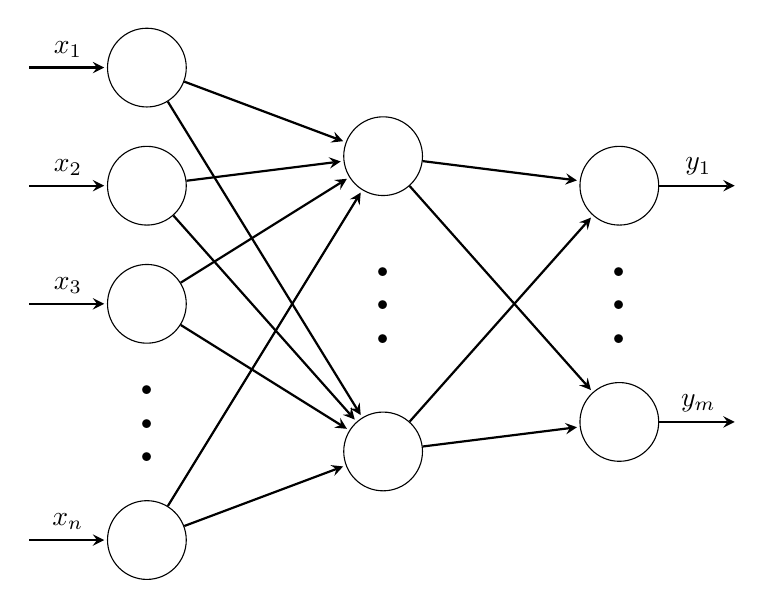
\begin{tikzpicture}
  [x=1.5cm, y=1.5cm, >=stealth, shorten >=1pt,
    every neuron/.style={
      circle,
      draw,
      minimum size=1cm
    },
    neuron missing/.style={
      draw=none, 
      scale=3,
      text height=0.333cm,
      execute at begin node=\color{black}$\vdots$
    },
  ]
% Draw input nodes
\foreach \m/\l [count=\y] in {1,2,3,missing,4}
  \node [every neuron/.try, neuron \m/.try] (input-\m) at (0,2.5-\y) {};

% Label input edges 
\foreach \l [count=\i] in {1,2,3,n}
  \draw [<-, shorten <=1pt, shorten >=0pt,thick] (input-\i) -- ++(-1,0)
  node [above, midway] {$x_\l$};

% Draw hidden nodes
\foreach \m [count=\y] in {1,missing,2}
  \node [every neuron/.try, neuron \m/.try ] (hidden-\m) at (2,2-\y*1.25) {};

% Draw output nodes
\foreach \m [count=\y] in {1,missing,2}
  \node [every neuron/.try, neuron \m/.try ] (output-\m) at (4,1.5-\y) {};

% Label output edges 
\foreach \l [count=\i] in {1,m}
  \draw [->,thick] (output-\i) -- ++(1,0)
  node [above, midway] {$y_\l$};

% Connect input nodes with hidden nodes
\foreach \i in {1,...,4}
  \foreach \j in {1,...,2}
    \draw [->,thick] (input-\i) -- (hidden-\j);

% Connect hidden nodes with output nodes
\foreach \i in {1,...,2}
  \foreach \j in {1,...,2}
    \draw [->,thick] (hidden-\i) -- (output-\j);
\end{tikzpicture}}
